\documentclass[a4paper,12pt]{article}
\usepackage{amsmath}
\usepackage{amsfonts}
\usepackage{textcomp}
\usepackage{amssymb}
\usepackage{graphicx}
\usepackage{fancyhdr}
\usepackage[spanish]{babel}
\usepackage[utf8]{inputenc}
\usepackage{array}
\usepackage[usenames,dvipsnames,svgnames,table]{xcolor}
\usepackage{multirow}


\definecolor{niceblue}{RGB}{60,110,190}

\usepackage{vmargin}
\setpapersize{A4}
\setmarginsrb{2.5cm}{1.5cm}{2.5cm}{2.5cm}
{1cm}{0cm}%
{1cm}{1cm}

\begin{document}

\begin{tabular}{ >{\centering\arraybackslash}m{4cm} >{\arraybackslash}m{8cm}}
\fbox{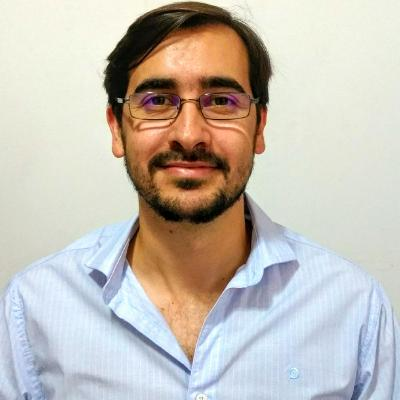
\includegraphics[width=25mm]{rodrigo}} & {\huge Dr. Rodrigo Baravalle} {\bf \em \color{CornflowerBlue} PostDoc (CONICET)}\\
\end{tabular}

\vspace{1cm}
\begin{tabular}{ll}
\bf{\color{Gray}Dirección} & Ocampo y Esmeralda, S2000EZP.\\
\bf{\color{Gray}Insitución} & CIFASIS, CONICET.\\
\bf{\color{Gray}Ciudad} & Rosario, Argentina\\
\bf{\color{Gray}Teléfono} & +54 341 4815569\\
\bf{\color{Gray}Fecha de Nacimiento}  & 20 April 1985\\
\bf{\color{Gray}Lugar de Nacimiento}  & Rosario, Santa Fe, Argentina\\
\bf{\color{Gray}Estado Civil}  & Soltero\\
\bf{\color{Gray}Correo Electrónico} &baravalle@cifasis-conicet.gov.ar\\
\end{tabular}
\vspace{1cm}

\section*{\color{niceblue} Sobre mí \rule{13.4cm}{2.2pt}}

\begin{small}
\noindent
Soy becario Postdoctoral en el Consejo Nacional de Investigaciones Científicas y Técnicas (CONICET). Mi lugar de trabajo es CIFASIS, Rosario, Argentina.
Mis intereses académicos incluyen Computación Gráfica - Modelado Procedimental - Síntesis de Texturas - Renderizado Foto-realista - Modelos Volumétricos - GPGPU - Lenguajes de shading y Fractales.
Adicionalmente, me gusta leer sobre astronomía, física y filosofía.
Eventualmente juego al ajedrez.
\end{small}


\section*{\color{niceblue} Educación \rule{12.8cm}{2.2pt}}

\begin{tabular}{lcp{9 cm}}
		\bf{2016} & & {\bf Doctor en Informática} (Modelado y Simulación Foto-Realística de Materiales). Facultad de Ciencias Exactas, Ingenier\'ia y Agrimensura - Universidad Nacional de Rosario. \\
		\bf{2010} & & {\bf Licenciado en Ciencias de la Computación}. Facultad de Ciencias Exactas, Ingenier\'ia y Agrimensura - Universidad Nacional de Rosario. Promedio Académico: 9.4 ``Distinguido''.\\
\end{tabular}

\newpage

\section*{\color{niceblue} Publicaciones \rule{12.3cm}{2.2pt}}

\subsection*{\color{niceblue} Revistas}

\begin{itemize}
\item {\bf Procedural bread making}. Rodrigo Baravalle, Gustavo Patow y Claudio Delrieux. En {\it Computers \& Graphics} {\bf 50}(2015):13-24. doi:10.1016/j.cag.2015.05.003.
\item {\bf Multifractal characterisation and classification of bread crumb digital images}. Rodrigo Baravalle, Claudio Delrieux and Juan Carlos Gómez. En {\it EURASIP Journal on Image and Video Processing}. {\bf 2015}:9. Abril 2015. doi:10.1186/s13640-015-0063-8.
\item {\bf Modelado para la renderización foto-realista de pan}. Rodrigo Baravalle, Leonardo Scandolo, Claudio Delrieux y Cristian García Bauza. En {\it Mecánica Computacional} ({\bf 33})26:1695-1709. Bariloche, Argentina. Septiembre 2014.
\item {\bf Bread crumb classification using fractal and multifractal features}. Rodrigo Baravalle, Claudio Delrieux y Juan Carlos G\'omez. En {\it Mecánica Computacional} ({\bf 31})17:3013-3025. Salta, Argentina. Noviembre 2012.
\end{itemize}

\subsection*{\color{niceblue} Reportes Técnicos Internacionales}
\begin{itemize}
\item {\bf 3D mapping of indoor environments with a time of flight camera}. Rodrigo Baravalle y Amaury N\`egre. E-MOTION (INRIA Grenoble Rh\^one-Alpes / LIG Laboratoire d'Informatique de Grenoble) Número: RT0406. Grenoble, Francia, Febrero 2011.
\end{itemize}

\subsection*{\color{niceblue} Conferencias}
\begin{itemize}
\item {\bf Experiencias con Cython y PyOpenCL}. En {\it Actas de la Segunda Conferencia de Python en la Ciencia}, SciPyConAr. Puerto Madryn, Argentina. Octubre 2014.
\item {\bf Imfractal: dimensiones Fractales con Python}.  En {\it Actas de la Primera Conferencia de Python en la Ciencia}, SciPyConAr. Puerto Madryn, Argentina. Mayo 2013.
\item {\bf Clasificación de muestras de pan por medio de extracción de características fractales}. Rodrigo Baravalle, Claudio Delrieux y Juan Carlos G\'omez. En {\it Actas de la quinta Escuela en Ciencias de las Imágenes}, ECIMAG. Santa Fe, Argentina, Julio 2012.
\item {\bf Síntesis procedimental de materiales: resultados en el modelado de pan y materiales cocidos}. Rodrigo Baravalle, Claudio Delrieux y Juan Carlos G\'omez. En {\it Actas del XIV Workshop de Investigadores en Ciencias de la Computación}, WICC. Posadas, Argentina, Abril 2012.
\item {\bf Síntesis de texturas utilizando sistemas de partículas}. Rodrigo Baravalle, Claudio Delrieux y Juan Carlos G\'omez. En {\it Actas de la cuarta Escuela en Ciencias de las Imágenes}, ECIMAG. Buenos Aires, Argentina, Agosto 2011.
\item {\bf Generación procedimental de contenido en el desarrollo de videojuegos}. Rodrigo Baravalle, Claudio Delrieux y Cristian Garc\'ia Bauza. En {\it Actas del primer Workshop Argentino de Video Juegos}, WAVi. Buenos Aires, Argentina, Diciembre 2010.
\item {\bf Un framework en GPU para representar y renderizar materiales en tiempo real}. Rodrigo Baravalle, Claudio Delrieux y Cristian Garc\'ia Bauza. En {\it Actas de la cuarta Escuela en Ciencias de las Imágenes}, ECIMAG. Bahía Blanca, Argentina, Julio 2010.
\end{itemize}


\subsection*{\color{niceblue} Tesis}
\begin{itemize}
\item {\bf Modelado y Simulación Foto-Realística de Materiales}. Rodrigo Baravalle, Claudio Delrieux y Juan Carlos Gómez. Tesis de Doctorado en Informática. Facultad de Ciencias Exactas, Ingeniería y Agrimensura, Universidad Nacional de Rosario, Argentina, 28 Marzo 2016.
\item {\bf Un framework en GPU para representar y renderizar materiales en tiempo real}. Rodrigo Baravalle, Claudio Delrieux y Cristian Garc\'ia Bauza. Tesis de Licenciatura en Ciencias de la Computación. Facultad de Ciencias Exactas, Ingeniería y Agrimensura, Universidad Nacional de Rosario, Argentina, 10 Agosto 2010.
\end{itemize}


\section*{\color{niceblue} Experiencia Docente \rule{10cm}{2.2pt}}

Adscripciones en diferentes materias de la carrera de grado "Licenciatura en Ciencias de la Computación" (Universidad Nacional de Rosario):
\begin{itemize}
\item Estructuras de Datos y Algoritmos I. Marzo - Agosto 2012.
\item Arquitectura del Computador. Septiembre 2012 - Febrero 2013.
\end{itemize}

\section*{\color{niceblue} Cursos Dictados \rule{11.3cm}{2.2pt}}
\begin{itemize}
\item {\bf Introducción a la Computación Gráfica} en el Departamento de Ciencias de la Computación (Rosario, Argentina. Noviembre-Diciembre 2014). Total: 10hs reloj.
\end{itemize}



\section*{\color{niceblue} Experiencia Laboral \rule{10.2cm}{2.2pt}}

\begin{itemize}
\item {\bf Pasantía de Investigación} en {\em IROBOT}, Pasadena, Estados Unidos, trabajando en segmentación de habitaciones para robots limpiadores de pisos. Septiembre 2015 - Diciembre 2015.
\item {\bf Pasantía de Investigación} en el grupo {\em E-MOTION, Inria}, Grenoble, Francia, trabajando en reconstrucción 3D. Septiembre 2010 - Febrero 2011.
\item {\bf Programador} en {\em E-ducativa}, Rosario, Argentina. Desarrollo web en Perl + Javascript. Septiembre 2008 - Agosto 2010.
\item {\bf Programador} en {\em UNR Campus Virtual}, Rosario, Argentina. Desarrollo web en PHP. Abril - Julio 2008.
\end{itemize}


\section*{\color{niceblue} Tesis de Grado Dirigidas \rule{9.3cm}{2.2pt}}
\begin{itemize}
\item {\bf Reconstrucción 3D densa sobre sistemas de SLAM basados en visión estéreo}. Ariel D'Alessandro, Co-Director. Universidad Nacional de Rosario, Argentina, {\it En progreso}.
\end{itemize}

\section*{\color{niceblue} Jurado de Tesis de Grado \rule{9cm}{2.2pt}}
\begin{itemize}
\item {\bf Aprendizaje Multiclase de Videoimágenes deportivas con Arquitecturas Profundas}. Martín Escarrá. Universidad Nacional de Rosario, Argentina. Febrero 2016.
\end{itemize}


\section*{\color{niceblue} Materias de Posgrado semestrales Aprobadas \rule{3cm}{2.2pt}}
\begin{itemize}
\item {\bf Procesamiento Digital de Imágenes}, Universidad Nacional de Rosario, Argentina. Dictada por el Dr. Guillermo Kaufmann, Phd. Nota Final: 9 (Nueve).
\item {\bf Computación Gráfica I}, UBA, Buenos Aires, Argentina. Dictada por el Dr. Claudio Delrieux, Phd. (UNS, Argentina). Nota Final: 10 (Diez).
\item {\bf Modelos Fractales y Sistemas Caóticos en Física Computacional y Ciencias Naturales}, DIEC, UNS, Bah\'ia Blanca, Argentina. Dictada por el Dr. Claudio Delrieux, Phd. (UNS, Argentina). Nota Final: 10 (Diez).
\end{itemize}


\section*{\color{niceblue} Disertaciones \rule{12.4cm}{2.2pt}}
\begin{itemize}
\item {\bf Modelado y Simulación Foto-Realística de Materiales}, Tesis Doctoral. Marzo 2016, Rosario, Argentina.
\item {\bf Modelado para la Renderización Foto-Realista de Pan}, en la $21^{a}$ ENIEF. Septiembre 2014, Bariloche, Argentina.
\item {\bf Bread Crumb Classification Using Fractal and Multifractal Features}, en la $10^{a}$ MECOM. Noviembre 2012, Salta, Argentina.
\item {\bf Síntesis de texturas utilizando sistemas de partículas}, en la $4^{a}$ ECImag. Agosto 2011, Buenos Aires, Argentina.
\item {\bf Un framework en GPU para representar y renderizar materiales en tiempo real}, en la $3^{a}$ ECImag. Julio 2010, Bahía Blanca, Argentina.
\end{itemize}

\section*{\color{niceblue} Cursos Tomados \rule{11.6cm}{2.2pt}}
\begin{itemize}
\item {\bf Análisis Fractal y Multifractal de Sistemas Complejos}, ECIMAG 2012. Dictado por: Dra. Tatijana Stosic (Universidade Federal Rural de Pernambuco, Recife, PE, Brazil).
\item {\bf Programación Paralela en GPU}, ECImag 2011. Dictado por: Dr. Juan Pablo D'amato (Universidad Nacional del Centro, Argentina).
\item {\bf Visualización de Superficies Algebraicas}, ECImag 2011. Dictada por: Dr. Andreas Matt (Mathematisches Forschungsinstitut Oberwolfach, Germany). Nota Final: 8 (Ocho).
\item {\bf A Practical Introduction to 3D Computer Vision}, ECImag 2010. Dictada por: Dr. Radim S\'ara (Politechnic Institute of Prague, Czech Republic).
\item {\bf Modelado Procedimental}, ECImag 2010. Dictada por: Dr. Gustavo Patow. (Grupo de Gráficos de Girona, España).
\item {\bf Patrones en el desarrollo de video-juegos}, ECImag 2009. Dictado por: Dr. Federico Balaguer (LIFIA, Universidad Nacional de La Plata, La Plata, Argentina).
\item {\bf Fractales: aplicaciones al procesamiento de imágenes y computación gráfica}, ECImag 2009. Dictado por: Dr. Claudio Delrieux (Universidad Nacional del Sur, Bah\'ia Blanca).
\item {\bf Procesamiento de Imágenes}, RIO 2007. Dictado por: Dr. Rafael Lins (Federal University of Pernambuco, Brazil). Nota Final: 10 (Diez).
\item {\bf Teoría de Categorías}, RIO 2007. Dictado por: Dr. Mat\'ias Menni (LIFIA, UNLP, Argentina).
\item {\bf Introducción a la computación cuántica}. Dictado por: Dr. Alejandro Diaz-Caro (Universidad Nacional de Rosario).
\end{itemize}

\section*{\color{niceblue} Becas Obtenidas \rule{11.8cm}{2.2pt}}

\begin{itemize}
\item Beca CONICET postdoctoral. Comienzo: Abril 2016. Duraci\'on: 2 a\~nos.
\item Beca CONICET de postgrado tipo II (Beca doctoral CONICET PG TII). Comienzo: Abril 2014. Duraci\'on: 2 a\~nos.
\item Beca CONICET de postgrado tipo I (Beca doctoral CONICET PG TI). Abril 2011 -Marzo 2014. Duraci\'on: 3 a\~nos.
\item Septiembre 2010 - Febrero 2011 - INRIA (Institut national de recherche en informatique et automatique), Grenoble, Francia. Tema: 3D Mapping.
\item 2008 - IMPA (Instituto de Matem\'atica Pura y Aplicada), R\'io de Janeiro, Brasil - Curso de verano en Computaci\'on Gr\'afica.
\end{itemize}

\section*{\color{niceblue} Participación en proyectos acreditados \rule{5.3cm}{2.2pt}}

\begin{itemize}
\item Enero 2013 - Diciembre 2016, {\bf Procesamiento de Señales Multimedia - Aplicaciones en Procesamiento Multimodal de Habla, Verificación Automática de Firmas Manuscritas, e Identificación de Sistemas No Lineales}. Identificador del proyecto: ING427. Acreditado por la Universidad Nacional de Rosario, Argentina.
\item Enero 2011 - Diciembre 2012, {\bf Procesamiento digital de imágenes - Aplicaciones en procesamiento audio-visual de habla, watermarking digital, reconocimiento automático de firmas manuscritas y reconocimiento de especies vegetales a partir de imágenes de nervaduras}. Identificador del proyecto: ING355. Acreditado por la Universidad Nacional de Rosario, Argentina.

\end{itemize}


\section*{\color{niceblue} Encuentros Científicos \rule{10cm}{2.2pt}}
\begin{small}
\begin{itemize}
\item $2^{a}$ ScipyConAr. Conferencia de Python en la Ciencia, Octubre 2014.
\item $21^{a}$ ENIEF, XXI Congreso sobre Métodos Numéricos y sus Aplicaciones, Septiembre 2014.
\item $1^{a}$ ScipyConAr. Conferencia de Python en la Ciencia, Mayo 2013.
\item $10^{o}$ MECOM. Congreso Argentino de Mec\'anica Computacional, Septiembre 2012.
\item $2^{a}$ EAGPGPU. Escuela Argentina de GPGPU Computing para Aplicaciones Cient\'ificas, Septiembre 2012.
\item $5^{a}$ ECImag. Escuela y Workshop de Ciencias de las Im\'agenes, Julio 2012.
\item $14^{o}$ WICC. Workshop de investigadores en Ciencias de la Computaci\'on, Abril 2012.
\item $4^{a}$ ECImag. Escuela y Workshop de Ciencias de las Im\'agenes, Agosto 2011.
\item $1^{a}$ PEAGPGPU. Primera Escuela Argentina de GPGPU Computing para Aplicaciones Cient\'ificas, Mayo 2011.
\item $3^{a}$ ECImag. Escuela y Workshop de Ciencias de las Im\'agenes, Julio 2010.
\item $7^{a}$ JCC, Rosario, Argentina, Octubre 2009.
\item $2^{a}$ ECImag. Escuela y Workshop de Ciencias de las Im\'agenes, Septiembre 2009.
\item $3^{er}$ STIC-AmSud, Seminario Cient\'ifico de Cooperaci\'on Franco-Sudamericana en
Ciencias y Tecnolog\'ias de la Inform\'atica y las Comunicaciones, Montevideo, Uruguay. Noviembre 2007.
\item $5^{a}$ JCC, Rosario, Argentina, Octubre 2007.
\item $14^{a}$ RIO, R\'io Cuarto, Argentina, Febrero 2007.
\item $2^{a}$ JAI, Rosario, Argentina, Diciembre 2006.
\item $4^{a}$ JCC, Rosario, Argentina, Octubre 2006.
\item $3^{a}$ JCC, Rosario, Argentina, Diciembre 2005.
\end{itemize}
\end{small}


\section*{\color{niceblue} Lenguajes \rule{13.2cm}{2.2pt}}

\begin{small}
\begin{description}
	\item[Español:] Nativo.
	\item[Inglés:] First Certificate In English (FCE) (Nivel B2), otorgado por la University of Cambridge, ESOL. Certificado número: 0026091410. Febrero 2010.
	\item[Francés:] DELF B2 (Nivel B2). Otorgado por la Alliance Fran\c{c}aise. Certificado número: 054041-201311T-2234032. Abril 2014.
	\item[Portugués:] Lectura.
\end{description}
\end{small}

\section*{\color{niceblue} Referencias \rule{12.9cm}{2.2pt}}

\begin{itemize}
\item {\bf Dr. Gustavo Patow}, PhD. Jefe del Grupo de Geometría y Gráficos (GGG), Girona, España.\\E-mail: dagush@imae.udg.edu \\
\item {\bf Dr. Claudio Delrieux}, PhD. Jefe del Departamento de Ingeniería Eléctrica y de Computadoras, Nacional del Sur, Argentina.\\E-mail: cad@uns.edu.ar\\
\item {\bf Dr. Mario Munich}, PhD. SVP Technology, IROBOT, Pasadena, EEUU.\\E-mail: mmunich@irobot.com. \\
\item {\bf Dr. Alexander Kleiner}, PhD. Senior Principal Robotics Scientist. IROBOT, Pasadena, EEUU.\\E-mail: alexander.kleiner@gmail.com. \\
\item {\bf Dr. Juan Carlos G\'omez}, PhD. Jefe del Laboratorio de Sistemas Dinámicos y Procesamiento de la Información, FCEIA, la Universidad Nacional de Rosario, Argentina.\\E-mail: jcgomez@fceia.unr.edu.ar\\
\item {\bf MSc. Amaury Nègre}, Ingeniero de Investigación en E-MOTION, Inria, Grenoble, Francia.\\E-mail: amaury.negre@inrialpes.fr. \\

\end{itemize}

\end{document}




